\documentclass{article}

\usepackage{amsmath}
\usepackage[utf8]{inputenc}
\usepackage{amssymb}
\usepackage{amsxtra}
\usepackage{listings}
\usepackage{graphicx}
\usepackage[labelfont=bf]{caption}

% TODO
% - Add references
% - Replace repeated text like "This allows the network ..."
% - Shorten descriptions of figures

\graphicspath{ {figures/} }

\newcommand{\refchapter}[1]{Chapter~\ref{#1}}
\newcommand{\refsec}[1]{Section~\ref{#1}}
\newcommand{\refeqn}[1]{Equation~(\ref{#1})}
\newcommand{\reffig}[1]{Figure~\ref{#1}}

\title{
  {\bf \scriptsize
    RHEINISCH-WESTF\"ALISCHE TECHNISCHE HOCHSCHULE AACHEN \\
    Neuroinspired Computing (Prof. Dr. Abigail Morrison)
  } \vspace{2cm} \\
  Deterministic Recurrent Neural Networks \\
  {\large Seminar Thesis} 
}
\author{Marco Bischoff (Matr.-Nr. 370222)}

\begin{document}


\pagestyle{headings}

\maketitle
\newpage

\tableofcontents
\newpage



\section{Introduction}
\label{ch:1}

Machine learning has seen a rapid evolution in recent years, with neural networks emerging
as a powerful tool for a wide range of applications. Initially inspired by the structure
and function of the human brain, artificial neural networks have evolved into a diverse
family of models, each tailored to specific tasks and data types. In particular, Recurrent
Neural Networks (RNNs) have revolutionized the processing of sequential data, enabling
tasks such as language modeling, machine translation, and speech recognition. In this
seminar thesis, we explore the foundational concepts, architectures, and applications of
RNNs, with a particular focus on the Long Short-Term Memory (LSTM) network and its role in
addressing the challenges of training RNNs.


\subsection{Feedforward Neural Networks}
\label{sec:1.0}

Before delving into the realm of RNNs, it is essential to understand the foundational
concepts of feedforward neural networks, which form the basis for more complex models such
as RNNs. Feedforward neural networks, also known as multilayer perceptrons, are a class of
neural networks that process input data through a series of interconnected layers. Each
layer consists of a set of nodes, or neurons, which perform a weighted sum of the inputs
followed by the application of an activation function. The output of each layer serves as
the input to the next layer, ultimately producing a final output. The process of training
a feedforward neural network involves adjusting the weights of the connections between
neurons to minimize the difference between the predicted and actual outputs, typically
using the backpropagation algorithm and gradient descent.

This poses a limitation on the types of data that can be processed by feedforward neural
networks, as they are designed to operate on fixed-size input vectors and produce
fixed-size output vectors. This constraint makes them ill-suited for tasks involving
sequential data, where the length of the input and output sequences may vary. For example,
in natural language processing, the length of a sentence can vary significantly, making it
challenging to process using a feedforward neural network. Additionally, feedforward
neural networks lack an internal state, meaning they do not have the ability to remember
information from previous inputs. This makes it difficult for them to capture the
sequential dependencies present in many real-world datasets. To address these limitations,
we turn to Recurrent Neural Networks.



\section{Recurrent Neural Networks}
\label{ch:2}

Recurrent Neural Networks (RNNs) are a class of neural networks that are designed to
handle sequential data by maintaining an internal state and processing input sequences one
element at a time. Unlike feedforward neural networks, which process the entire input at
once, RNNs process the input elements sequentially, allowing them to capture dependencies
over time. This makes them well-suited for tasks such as language modeling, machine
translation, and speech recognition, where the order of the input elements is crucial for
understanding the data.

\begin{figure}[htbp]
  \centering
  \includegraphics[width=0.9\textwidth]{RNN Unrolled.drawio.png}
  \caption{A recurrent neural network unrolled into a sequence of layers. The input
    sequence $x_0, x_1, \ldots, x_t$ is shown in blue, the network layer in green and the
    output sequence $y_0, y_1, \ldots, y_t$ in purple.}
  \label{fig:rnn-unrolled}
\end{figure}

In its simplest form, the structure of an RNN is the same as a feedforward neural network,
with the addition of a feedback loop that allows the network to maintain an internal
state. This internal state is updated at each time step, allowing the network to remember
information from previous inputs. The output of the network at each time step is
influenced not only by the current input but also by the internal state, which captures
the context from previous inputs. This means that, instead of having multiple layers with
separate weights, RNNs have a single layer that acts as a dynamical system, changing over
time. The repeating module in an RNN can be unrolled into a sequence of interconnected
layers, allowing the network to process sequences of arbitrary length, as shown in
\reffig{fig:rnn-unrolled}. This unrolling reveals that RNNs are intimately related to
sequences and lists, making them a natural architecture for processing data of this form.

\subsection{Categories of Applications}
\label{sec:2.0}

\begin{figure}[htbp]
  \centering
  \includegraphics[width=0.9\textwidth]{Karpathy application types.jpeg}
  \caption{Ways of applying RNNs to different types of data. Both the input and output can
    be a fixed-size vector or a sequence of vectors. If both are sequences, the input and
    output vectors can either be regarded as pairs or as unrelated sequences of different
    lengths. \cite{karpathyUnreasonableEffectivenessRecurrent}}
  \label{fig:rnn-application-types}
\end{figure}

The applications of RNNs can be categorized based on the length of the input and output
sequences and the relationship between them, as shown in
\reffig{fig:rnn-application-types}. For example, for tasks such as image classification,
where the input and output sequences are of fixed length, RNNs can be used in a manner
similar to feedforward neural networks (one-to-one). They can also be used for tasks such
as image captioning, where the input is a fixed-size image and the output is a sequence of
words (one-to-many). Additionally, RNNs can be used for tasks such as sentiment analysis,
where the input is a sequence of words and the output is a single value (many-to-one).
Tasks, where both the input and output are sequences of varying lengths (many-to-many),
can be categorized into two subtypes. For example, in machine translation, the input
sequence is processed first, and then the output sequence is generated. In contrast, for
video classification, the output is generated simultaneously with the input, allowing the
network to use the previous frames as context. This demonstrates the flexibility of RNNs
in handling a wide range of tasks involving sequential data.

% Possible extensions: Sequential processing in absence of sequences


\subsection{Internal Structure}
\label{sec:2.1}

\begin{figure}[htbp]
  \centering
  \includegraphics[width=0.9\textwidth]{Block Diagram Feedforward.drawio.png}
  \caption{The internal structure of a feedforward neural network with a single layer. The
    input vector $x$ is transformed by a linear transformation $Wx + b$ and then passed
    through an activation function. The output can, for example, be processed with another
    linear transformation and a softmax function to produce a probability distribution
    over classes. The vector $y$ is the output of the network. In a multi-layer network,
    the components in the green box would be repeated for each layer.}
  \label{fig:internal-feedforward}
\end{figure}

\begin{figure}[htbp]
  \centering
  \includegraphics[width=0.9\textwidth]{Block Diagram RNN.drawio.png}
  \caption{The internal structure of a recurrent neural network with a single layer. The
    input vector $x$ and the previous state vector $h_{t-1}$ are concatenated and
    transformed by a linear transformation and an activation function to produce the new
    state vector $h_t$. To produce the output vector $y_t$, the state vector can, for
    example, be transformed by another linear transformation and a softmax function.}
  \label{fig:internal-rnn}
\end{figure}

To understand the internal structure of an RNN, we compare a single layer feedforward NN
with a single layer RNN. As shown in \reffig{fig:internal-feedforward}, a feedforward NN
transforms the input vector $x$ by a linear transformation and an activation function to
produce the output of a single layer. In contrast, as shown in \reffig{fig:internal-rnn},
an RNN first concatenates the input vector $x$ with the previous state vector $h_{t-1}$,
then transforms the concatenated vector in the same way as a feedforward NN. The resulting
state vector $h_t$ then serves as the input to the next time step. For the first iteration
of the RNN, the previous state vector is typically initialized to a vector of zeros.
However, it can also be learned as part of the training process, which can boost the
performance of the network in some cases.


\subsection{Backpropagation}
\label{sec:2.2}

% First, introduce regular backpropagation
The training of RNNs is typically performed using the backpropagation through time (BPTT)
algorithm, which is an extension of the backpropagation algorithm used to train
feedforward neural networks. As an example, consider a single layer feedforward NN, like
the green box in \reffig{fig:internal-feedforward}. Let
\begin{itemize}
  \item $x$ be the input vector,
  \item $W$ the weight matrix,
  \item $b$ the bias vector,
  \item $y$ the output vector,
  \item $t$ the target vector (ground truth)
  \item $\sigma$ the activation function, and
  \item $L = \frac{1}{2} \sum_{i=1}^{n} (t_i - y_i)^2$ the loss function (e.g. mean
        squared error).
\end{itemize}
We first do a forward pass to compute the output $y = \sigma(Wx + b)$ and compare it to
the target $t$ by the loss function $L$. Then, we do a backward pass to compute the
gradient of the loss function with respect to the weights and biases of the network. Here,
we use the chain rule of calculus:
\begin{align}
  \frac{\partial L}{\partial W} & = \frac{\partial L}{\partial y} \frac{\partial y}{\partial W}                                             \\
                                & = \frac{\partial L}{\partial y} \frac{\partial y}{\partial (Wx + b)} \frac{\partial (Wx + b)}{\partial W} \\
                                & = -(t-y) \cdot \sigma'(Wx + b) \cdot x^T
\end{align}
The gradient for the bias vector $\frac{\partial L}{\partial b}$ can be computed
similarly. For a network with multiple layers, the gradients are computed layer by layer
using the chain rule, starting from the output layer and moving backwards through the
network. In the final step, the weights and biases are updated in the direction that
minimizes the loss: $W \leftarrow W - \alpha \frac{\partial L}{\partial W}$ and $b
  \leftarrow b - \alpha \frac{\partial L}{\partial b}$, where $\alpha$ is the learning rate.
This is usually done using an optimization algorithm such as stochastic gradient descent.

% Then, explain how BPTT differs
The BPTT algorithm extends this approach to RNNs by unrolling the network into a sequence
of interconnected layers, as shown in \reffig{fig:rnn-unrolled}. The forward pass is
performed as usual, with the output of each time step serving as the input to the next
time step. The backward pass then accumulates the gradients over the entire sequence and
updates the weights and biases accordingly. This allows the network to capture the
dependencies between the input elements and learn from the entire sequence, rather than
just the current input. The key difference between BPTT and regular backpropagation is
that the weights of the RNN are shared across time steps, meaning that the same weights
are used at each time step. Also, the number of time steps is not given by the number of
layers, but by the length of the input sequence. For long sequences, this can lead to
problems such as vanishing or exploding gradients, which can make training difficult.


\subsection{The Problem of Long-Term Dependencies}
\label{sec:2.3}

One of the key challenges in training RNNs is the problem of long-term dependencies. To
illustrate this, consider a simplified RNN \cite{pascanuDifficultyTrainingRecurrent2013}
that takes an input sequence $x_0, x_1, \ldots, x_n$ and produces a sequence of
outputs/hidden states $h_0, h_1, \ldots, h_n$. It is defined by the function $F$ for each
time step $t \in \{0, 1, \ldots, n\}$:
\begin{equation}
  h_t = F(h_{t-1}, x_t) = W_h \tanh{h_{t-1}} + W_x x_t + b
\end{equation}
Then the gradient with respect to the hidden state at time step $t$ is given by:
\begin{equation}
  \label{eq:gradient-hidden-state}
  \nabla_h F(h_{t-1}, x_t) = W_h \text{diag}(\tanh'(h_{t-1}))
\end{equation}
For the backward pass, we need to compute the gradient of the loss function, which in
this case is given by
\begin{equation}
  \partial L = \nabla_h L(h_n, x_1, \ldots, x_n) \cdot \sum_{t=1}^{n} \prod_{k=n-t+1}^{n} \nabla_h F(h_{k-1}, x_k)
\end{equation}
where each term in the sum is the gradient of the current layer. The sum can be written
as:
\begin{align}
   & \sum_{t=1}^{n} \prod_{k=n-t+1}^{n} \nabla_h F(h_{k-1}, x_k)                                      \label{eq:gradient-sum} \\
   & = \nabla_h F(h_{n-1}, x_n)                                                                       \nonumber               \\
   & + \nabla_h F(h_{n-1}, x_n) \cdot \nabla_h F(h_{n-2}, x_{n-1})                                    \nonumber               \\
   & + \nabla_h F(h_{n-1}, x_n) \cdot \nabla_h F(h_{n-2}, x_{n-1}) \cdot \nabla_h F(h_{n-3}, x_{n-2}) \nonumber               \\
   & + \ldots \nonumber
\end{align}
With \refeqn{eq:gradient-hidden-state} and \refeqn{eq:gradient-sum}, we can see that the
gradient for time step $t$ is predominantly influenced by $W_h^{n-t+1}$. If the largest
singular value of $W_h$ is less than 1, the gradient will vanish as $t$ increases. If it
is greater than 1, the gradient will explode
\cite{pascanuDifficultyTrainingRecurrent2013}. This makes it difficult for the network to
learn long-term dependencies, as the gradients become too small or too large to be useful.
This is known as the problem of long-term dependencies, and it is a fundamental limitation
of standard RNNs.

Multiple approaches have been proposed to address this problem, for example, clipping the
gradient to prevent it from becoming too large
\cite{pascanuDifficultyTrainingRecurrent2013}. Let $\nabla_W L$ be the gradient of the
loss function and $\epsilon$ a small constant. Then the clipped gradient $\nabla$ is
\begin{equation}
  \nabla =
  \begin{cases}
    \nabla_W L                                       & \text{if } ||\nabla_W L|| < \epsilon \\
    \epsilon \cdot \frac{\nabla_W L}{||\nabla_W L||} & \text{otherwise}
  \end{cases}
\end{equation}
This prevents the gradient from becoming too large, but it does not address the problem of
vanishing gradients. Another approach is to use ReLU activation functions
\cite{glorotDeepSparseRectifier2010}, which have the advantage of not saturating for
positive inputs because their derivative is 1. However, the problem of vanishing gradients
still remains for negative inputs. Moreover, there were methods proposed to initialize the
weights of the network in a way that prevents the gradients from vanishing or exploding
\cite{kumar2017weight}. While these methods can mitigate the problem of long-term
dependencies to some extent, they do not provide a complete solution. A more effective
approach is to use Long Short-Term Memory (LSTM) networks, which were specifically
developed to address the problem of vanishing and exploding gradients in RNNs.



\section{Long Short-Term Memory Networks}
\label{ch:3}

Long Short-Term Memory (LSTM) networks are a special type of RNN that are designed to
learn long-term dependencies more effectively than standard RNNs. They were introduced by
Hochreiter and Schmidhuber in 1997 \cite{hochreiterLongShorttermMemory1997} and have since
become a popular choice for a wide range of applications, including language modeling,
machine translation, and speech recognition. The key idea behind LSTMs is the use of a
memory cell, which allows the network to store and access information over long time
scales. In this section, we explore the architecture and operation of LSTMs, as well as
their applications and variants.


\subsection{Architecture}
\label{sec:3.0}

\begin{figure}
  \centering
  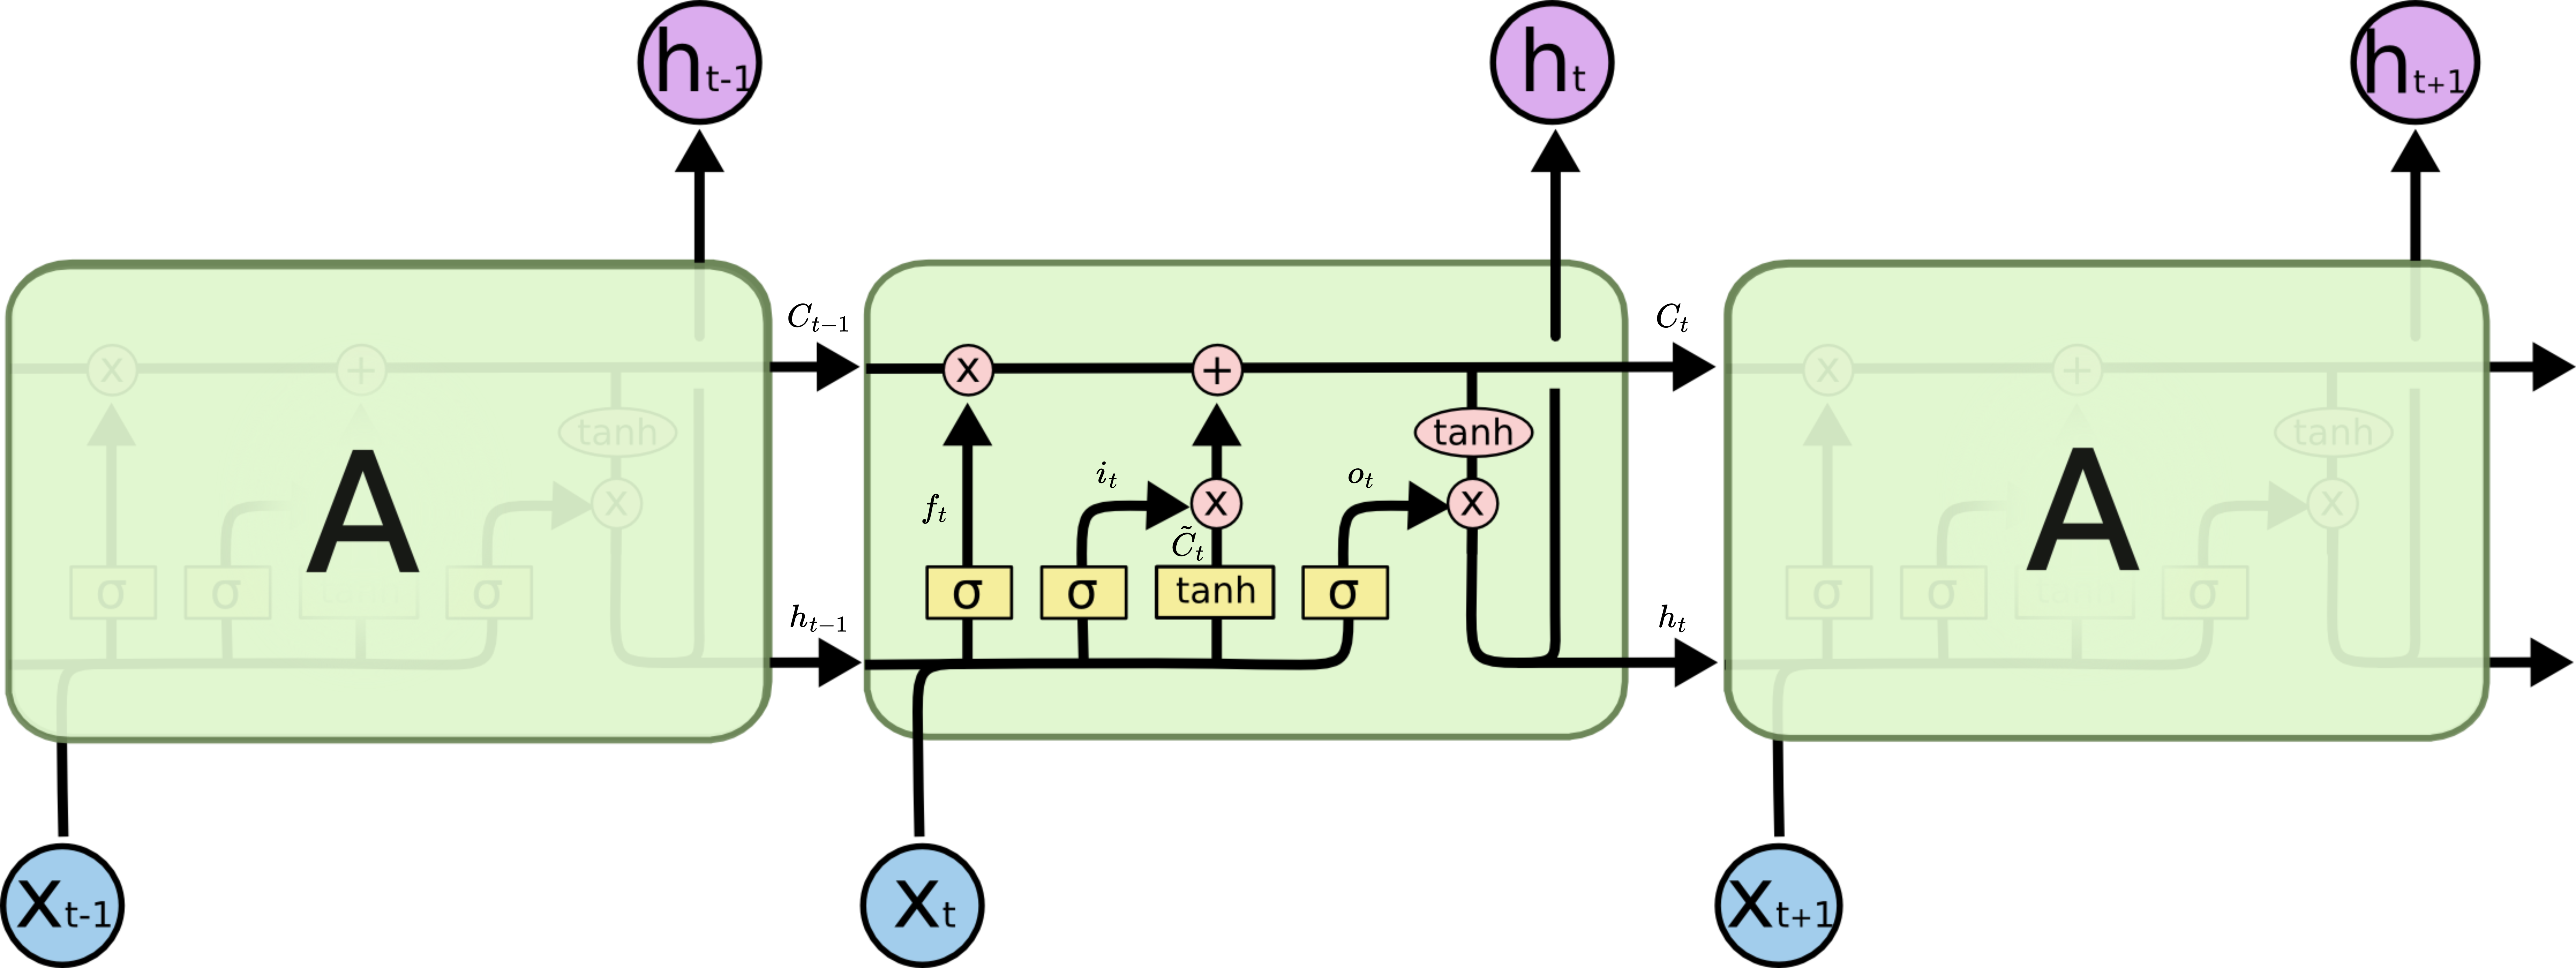
\includegraphics[width=0.9\textwidth]{LSTM Architecture.drawio.png}
  \caption{The repeating module of an LSTM network. Each yellow box represents a neural
    network layer with its activation function and the pink circles represent pointwise
    operations. The lines merging denote concatenation, while a line forking denotes its
    content being copied. The output is denoted by $h_t$. \cite{olahUnderstandingLSTM}}
  \label{fig:lstm}
\end{figure}

The architecture of an LSTM network is based on a repeating module that contains four
interacting layers, as shown in \reffig{fig:lstm}. The key to LSTMs is the cell state
$C_t$, which runs straight down the entire chain with only minor linear interactions. This
allows information to flow along the cell state unchanged, making it easy for the network
to remember information over long time scales. The cell state is regulated by structures
called gates, which are composed of neural network layers and pointwise operations. The
gates allow the network to control the flow of information into and out of the cell state,
enabling it to remember or forget information as needed.


\subsubsection{Forget Gate}
\label{sec:3.0.0}

The first step in the operation of an LSTM is to decide what information to forget from
the cell state. This is done by a sigmoid layer called the forget gate layer, which takes
the previous hidden state $h_{t-1}$ and the current input $x_t$ as input and outputs a
number between $0$ and $1$ for each element in the cell state $C_{t-1}$. A value of $0$
indicates that the corresponding element should be forgotten, while a value of $1$
indicates that it should be retained. This allows the network to selectively forget
information from the cell state as needed, enabling it to discard irrelevant information
and focus on the most important elements.
\begin{equation}
  f_t = \sigma(W_f \cdot [h_{t-1}, x_t] + b_f)
\end{equation}


\subsubsection{Input Gate}
\label{sec:3.0.1}

The next step is to decide what new information to store in the cell state. This has two
parts. First, a sigmoid layer called the input gate layer decides which values to update.
Next, a tanh layer creates a vector of new candidate values $\tilde{C}_t$ that could be
added to the state. The input gate layer outputs a number between $0$ and $1$ for each
element in the cell state, indicating how much of the new candidate values should be added
to the state. This allows the network to selectively update the cell state with new
information, enabling it to incorporate relevant information from the current input.
\begin{align}
  i_t         & = \sigma(W_i \cdot [h_{t-1}, x_t] + b_i) \\
  \tilde{C}_t & = \tanh(W_C \cdot [h_{t-1}, x_t] + b_C)
\end{align}


\subsubsection{Update Cell State}
\label{sec:3.0.2}

The next step is to update the old cell state $C_{t-1}$ into the new cell state $C_t$. The
previous steps have already decided what to do, so the network just needs to actually do
it. First, the old state is multiplied by the forget gate $f_t$, forgetting the things
that were decided to forget earlier. Then, the new candidate values $\tilde{C}_t$ are added
to the state, scaled by how much the input gate decided to update each state value.
\begin{equation}
  C_t = f_t \cdot C_{t-1} + i_t \cdot \tilde{C}_t
\end{equation}


\subsubsection{Output Gate}
\label{sec:3.0.3}

Finally, the network needs to decide what to output. This output will be based on the cell
state, but will be a filtered version. First, a sigmoid layer called the output gate layer
decides what parts of the cell state should be output. Then, the cell state is put through
a tanh function to push the values to be between $-1$ and $1$, and multiplied by the
output of the sigmoid gate. The result is the output of the network at the current time
step $h_t$, which can be used for further processing or as the final output of the
network.
\begin{align}
  o_t & = \sigma(W_o \cdot [h_{t-1}, x_t] + b_o) \\
  h_t & = o_t \cdot \tanh(C_t)
\end{align}


\subsection{Variants}
\label{sec:3.1}

LSTMs have been the subject of extensive research, leading to the development of several
variants that aim to improve their performance and address specific challenges
\cite{greffLSTMSearchSpace2017}. One popular variant, introduced by Gers and Schmidhuber
in 2000 \cite{gersRecurrentNetsTime2000}, adds peephole connections to the architecture
of the LSTM. These connections allow the cell to control the gates more precisely, making
it easier for the network to learn precise timings. Additionally, the output activation
function is omitted, as there is no evidence that it is essential for solving the problems
that LSTMs have been tested on so far.

% Variant: Dynamic Cortex Memory
% TODO: This is copy paste from the abstract
Another variant, called Dynamic Cortex Memory (DCM), was introduced by Otte et al. in 2014
\cite{otte2014dynamic}. The DCM is an extension of the LSTM model that enhances the inner
interplay of the gates and the error carousel due to several new and trainable
connections. These connections enable a direct signal transfer from the gates to one
another, allowing the network to converge faster during training with backpropagation
through time (BPTT) than LSTM under the same training conditions. Furthermore, DCMs yield
better generalization results than LSTMs, as shown for different supervised problem
scenarios, including storing precise values, adding, and learning a context-sensitive
grammar.

% Variant: Gated Recurrent Unit

\begin{figure}[htbp]
  \centering
  \includegraphics[width=0.9\textwidth]{LSTM3-var-GRU.png}
  \caption{The structure of a Gated Recurrent Unit (GRU) network. \cite{olahUnderstandingLSTM}}
  \label{fig:gru}
\end{figure}
One of the most well-known variants of the LSTM architecture is the Gated Recurrent Unit
(GRU), which was proposed by Cho et al. in 2014
\cite{choLearningPhraseRepresentations2014}. The GRU simplifies the LSTM architecture by
removing the output gate and the cell state, and combining the input and forget gates into
a single update gate. This reduces the number of parameters in the network and makes it
easier to train. The internal structure of a GRU network is shown in \reffig{fig:gru}.
While the GRU has been shown to perform comparably to the LSTM on many tasks, it has the
advantage of being simpler and more efficient, making it a popular choice for many
applications.





% ########################################################################################
% Blog post: Understanding LSTM Networks, by Christopher Olah
% ########################################################################################

% Recurrent Neural Networks

% Humans don’t start their thinking from scratch every second. As you read this essay, you
% understand each word based on your understanding of previous words. You don’t throw
% everything away and start thinking from scratch again. Your thoughts have persistence.

% Traditional neural networks can’t do this, and it seems like a major shortcoming. For
% example, imagine you want to classify what kind of event is happening at every point in a
% movie. It’s unclear how a traditional neural network could use its reasoning about
% previous events in the film to inform later ones.

% Recurrent neural networks address this issue. They are networks with loops in them,
% allowing information to persist.


% Recurrent Neural Networks have loops. In the above diagram, a chunk of neural network, A ,
% looks at some input xt and outputs a value ht . A loop allows information to be passed
% from one step of the network to the next.

% These loops make recurrent neural networks seem kind of mysterious. However, if you think
% a bit more, it turns out that they aren’t all that different than a normal neural network.
% A recurrent neural network can be thought of as multiple copies of the same network, each
% passing a message to a successor. Consider what happens if we unroll the loop:

% An unrolled recurrent neural network. An unrolled recurrent neural network. This
% chain-like nature reveals that recurrent neural networks are intimately related to
% sequences and lists. They’re the natural architecture of neural network to use for such
% data.

% And they certainly are used! In the last few years, there have been incredible success
% applying RNNs to a variety of problems: speech recognition, language modeling,
% translation, image captioning… The list goes on. I’ll leave discussion of the amazing
% feats one can achieve with RNNs to Andrej Karpathy’s excellent blog post, The Unreasonable
% Effectiveness of Recurrent Neural Networks. But they really are pretty amazing.

% Essential to these successes is the use of “LSTMs,” a very special kind of recurrent
% neural network which works, for many tasks, much much better than the standard version.
% Almost all exciting results based on recurrent neural networks are achieved with them.
% It’s these LSTMs that this essay will explore.

% The Problem of Long-Term Dependencies One of the appeals of RNNs is the idea that they
% might be able to connect previous information to the present task, such as using previous
% video frames might inform the understanding of the present frame. If RNNs could do this,
% they’d be extremely useful. But can they? It depends.

% Sometimes, we only need to look at recent information to perform the present task. For
% example, consider a language model trying to predict the next word based on the previous
% ones. If we are trying to predict the last word in “the clouds are in the sky,” we don’t
% need any further context – it’s pretty obvious the next word is going to be sky. In such
% cases, where the gap between the relevant information and the place that it’s needed is
% small, RNNs can learn to use the past information.


% But there are also cases where we need more context. Consider trying to predict the last
% word in the text “I grew up in France… I speak fluent French.” Recent information suggests
% that the next word is probably the name of a language, but if we want to narrow down which
% language, we need the context of France, from further back. It’s entirely possible for the
% gap between the relevant information and the point where it is needed to become very
% large.

% Unfortunately, as that gap grows, RNNs become unable to learn to connect the information.

% Neural networks struggle with long term dependencies. In theory, RNNs are absolutely
% capable of handling such “long-term dependencies.” A human could carefully pick parameters
% for them to solve toy problems of this form. Sadly, in practice, RNNs don’t seem to be
% able to learn them. The problem was explored in depth by Hochreiter (1991) [German] and
% Bengio, et al. (1994), who found some pretty fundamental reasons why it might be
% difficult.

% Thankfully, LSTMs don’t have this problem!

% LSTM Networks Long Short Term Memory networks – usually just called “LSTMs” – are a
% special kind of RNN, capable of learning long-term dependencies. They were introduced by
% Hochreiter & Schmidhuber (1997), and were refined and popularized by many people in
% following work.1 They work tremendously well on a large variety of problems, and are now
% widely used.

% LSTMs are explicitly designed to avoid the long-term dependency problem. Remembering
% information for long periods of time is practically their default behavior, not something
% they struggle to learn!

% All recurrent neural networks have the form of a chain of repeating modules of neural
% network. In standard RNNs, this repeating module will have a very simple structure, such
% as a single tanh layer.


% The repeating module in a standard RNN contains a single layer. LSTMs also have this chain
% like structure, but the repeating module has a different structure. Instead of having a
% single neural network layer, there are four, interacting in a very special way.

% A LSTM neural network. The repeating module in an LSTM contains four interacting layers.
% Don’t worry about the details of what’s going on. We’ll walk through the LSTM diagram step
% by step later. For now, let’s just try to get comfortable with the notation we’ll be
% using.


% In the above diagram, each line carries an entire vector, from the output of one node to
% the inputs of others. The pink circles represent pointwise operations, like vector
% addition, while the yellow boxes are learned neural network layers. Lines merging denote
% concatenation, while a line forking denote its content being copied and the copies going
% to different locations. The Core Idea Behind LSTMs The key to LSTMs is the cell state, the
% horizontal line running through the top of the diagram.

% The cell state is kind of like a conveyor belt. It runs straight down the entire chain,
% with only some minor linear interactions. It’s very easy for information to just flow
% along it unchanged.


% The LSTM does have the ability to remove or add information to the cell state, carefully
% regulated by structures called gates.

% Gates are a way to optionally let information through. They are composed out of a sigmoid
% neural net layer and a pointwise multiplication operation.


% The sigmoid layer outputs numbers between zero and one, describing how much of each
% component should be let through. A value of zero means “let nothing through,” while a
% value of one means “let everything through!”

% An LSTM has three of these gates, to protect and control the cell state.

% Step-by-Step LSTM Walk Through The first step in our LSTM is to decide what information
% we’re going to throw away from the cell state. This decision is made by a sigmoid layer
% called the “forget gate layer.” It looks at ht−1 and xt , and outputs a number between 0
% and 1 for each number in the cell state Ct−1 . A 1 represents “completely keep this” while
% a 0 represents “completely get rid of this.”

% Let’s go back to our example of a language model trying to predict the next word based on
% all the previous ones. In such a problem, the cell state might include the gender of the
% present subject, so that the correct pronouns can be used. When we see a new subject, we
% want to forget the gender of the old subject.


% The next step is to decide what new information we’re going to store in the cell state.
% This has two parts. First, a sigmoid layer called the “input gate layer” decides which
% values we’ll update. Next, a tanh layer creates a vector of new candidate values, C~t ,
% that could be added to the state. In the next step, we’ll combine these two to create an
% update to the state.

% In the example of our language model, we’d want to add the gender of the new subject to
% the cell state, to replace the old one we’re forgetting.


% It’s now time to update the old cell state, Ct−1 , into the new cell state Ct . The
% previous steps already decided what to do, we just need to actually do it.

% We multiply the old state by ft , forgetting the things we decided to forget earlier. Then
% we add it∗C~t . This is the new candidate values, scaled by how much we decided to update
% each state value.

% In the case of the language model, this is where we’d actually drop the information about
% the old subject’s gender and add the new information, as we decided in the previous steps.


% Finally, we need to decide what we’re going to output. This output will be based on our
%  cell state, but will be a filtered version. First, we run a sigmoid layer which decides
%  what parts of the cell state we’re going to output. Then, we put the cell state through
%  tanh (to push the values to be between −1 and 1 ) and multiply it by the output of the
%  sigmoid gate, so that we only output the parts we decided to.

% For the language model example, since it just saw a subject, it might want to output
% information relevant to a verb, in case that’s what is coming next. For example, it might
% output whether the subject is singular or plural, so that we know what form a verb should
% be conjugated into if that’s what follows next.


% Variants on Long Short Term Memory What I’ve described so far is a pretty normal LSTM. But
% not all LSTMs are the same as the above. In fact, it seems like almost every paper
% involving LSTMs uses a slightly different version. The differences are minor, but it’s
% worth mentioning some of them.

% One popular LSTM variant, introduced by Gers & Schmidhuber (2000), is adding “peephole
% connections.” This means that we let the gate layers look at the cell state.


% The above diagram adds peepholes to all the gates, but many papers will give some
% peepholes and not others.

% Another variation is to use coupled forget and input gates. Instead of separately deciding
% what to forget and what we should add new information to, we make those decisions
% together. We only forget when we’re going to input something in its place. We only input
% new values to the state when we forget something older.


% A slightly more dramatic variation on the LSTM is the Gated Recurrent Unit, or GRU,
% introduced by Cho, et al. (2014). It combines the forget and input gates into a single
% “update gate.” It also merges the cell state and hidden state, and makes some other
% changes. The resulting model is simpler than standard LSTM models, and has been growing
% increasingly popular.

% A gated recurrent unit neural network. These are only a few of the most notable LSTM
% variants. There are lots of others, like Depth Gated RNNs by Yao, et al. (2015). There’s
% also some completely different approach to tackling long-term dependencies, like Clockwork
% RNNs by Koutnik, et al. (2014).

% Which of these variants is best? Do the differences matter? Greff, et al. (2015) do a nice
% comparison of popular variants, finding that they’re all about the same. Jozefowicz, et
% al. (2015) tested more than ten thousand RNN architectures, finding some that worked
% better than LSTMs on certain tasks.

% Conclusion Earlier, I mentioned the remarkable results people are achieving with RNNs.
% Essentially all of these are achieved using LSTMs. They really work a lot better for most
% tasks!

% Written down as a set of equations, LSTMs look pretty intimidating. Hopefully, walking
% through them step by step in this essay has made them a bit more approachable.

% LSTMs were a big step in what we can accomplish with RNNs. It’s natural to wonder: is
% there another big step? A common opinion among researchers is: “Yes! There is a next step
% and it’s attention!” The idea is to let every step of an RNN pick information to look at
% from some larger collection of information. For example, if you are using an RNN to create
% a caption describing an image, it might pick a part of the image to look at for every word
% it outputs. In fact, Xu, et al. (2015) do exactly this – it might be a fun starting point
% if you want to explore attention! There’s been a number of really exciting results using
% attention, and it seems like a lot more are around the corner…

% Attention isn’t the only exciting thread in RNN research. For example, Grid LSTMs by
% Kalchbrenner, et al. (2015) seem extremely promising. Work using RNNs in generative models
% – such as Gregor, et al. (2015), Chung, et al. (2015), or Bayer & Osendorfer (2015) – also
% seems very interesting. The last few years have been an exciting time for recurrent neural
% networks, and the coming ones promise to only be more so!




% ########################################################################################
% Blog post: The Unreasonable Effectiveness of Recurrent Neural Networks, by Andrej Karpathy
% ########################################################################################

% There’s something magical about Recurrent Neural Networks (RNNs). I still remember when
% I trained my first recurrent network for Image Captioning. Within a few dozen minutes of
% training my first baby model (with rather arbitrarily-chosen hyperparameters) started to
% generate very nice looking descriptions of images that were on the edge of making sense.
% Sometimes the ratio of how simple your model is to the quality of the results you get
% out of it blows past your expectations, and this was one of those times. What made this
% result so shocking at the time was that the common wisdom was that RNNs were supposed to
% be difficult to train (with more experience I’ve in fact reached the opposite
% conclusion). Fast forward about a year: I’m training RNNs all the time and I’ve
% witnessed their power and robustness many times, and yet their magical outputs still
% find ways of amusing me. This post is about sharing some of that magic with you.

% We’ll train RNNs to generate text character by character and ponder the question “how is
% that even possible?”

% By the way, together with this post I am also releasing code on Github that allows you
% to train character-level language models based on multi-layer LSTMs. You give it a large
% chunk of text and it will learn to generate text like it one character at a time. You
% can also use it to reproduce my experiments below. But we’re getting ahead of ourselves;
% What are RNNs anyway?

% Recurrent Neural Networks Sequences. Depending on your background you might be
% wondering: What makes Recurrent Networks so special? A glaring limitation of Vanilla
% Neural Networks (and also Convolutional Networks) is that their API is too constrained:
% they accept a fixed-sized vector as input (e.g. an image) and produce a fixed-sized
% vector as output (e.g. probabilities of different classes). Not only that: These models
% perform this mapping using a fixed amount of computational steps (e.g. the number of
% layers in the model). The core reason that recurrent nets are more exciting is that they
% allow us to operate over sequences of vectors: Sequences in the input, the output, or in
% the most general case both. A few examples may make this more concrete:


% Each rectangle is a vector and arrows represent functions (e.g. matrix multiply). Input
% vectors are in red, output vectors are in blue and green vectors hold the RNN's state
% (more on this soon). From left to right: (1) Vanilla mode of processing without RNN,
% from fixed-sized input to fixed-sized output (e.g. image classification). (2) Sequence
% output (e.g. image captioning takes an image and outputs a sentence of words). (3)
% Sequence input (e.g. sentiment analysis where a given sentence is classified as
% expressing positive or negative sentiment). (4) Sequence input and sequence output (e.g.
% Machine Translation: an RNN reads a sentence in English and then outputs a sentence in
% French). (5) Synced sequence input and output (e.g. video classification where we wish
% to label each frame of the video). Notice that in every case are no pre-specified
% constraints on the lengths sequences because the recurrent transformation (green) is
% fixed and can be applied as many times as we like. As you might expect, the sequence
% regime of operation is much more powerful compared to fixed networks that are doomed
% from the get-go by a fixed number of computational steps, and hence also much more
% appealing for those of us who aspire to build more intelligent systems. Moreover, as
% we’ll see in a bit, RNNs combine the input vector with their state vector with a fixed
% (but learned) function to produce a new state vector. This can in programming terms be
% interpreted as running a fixed program with certain inputs and some internal variables.
% Viewed this way, RNNs essentially describe programs. In fact, it is known that RNNs are
% Turing-Complete in the sense that they can to simulate arbitrary programs (with proper
% weights). But similar to universal approximation theorems for neural nets you shouldn’t
% read too much into this. In fact, forget I said anything.

% If training vanilla neural nets is optimization over functions, training recurrent nets
% is optimization over programs.

% Sequential processing in absence of sequences. You might be thinking that having
% sequences as inputs or outputs could be relatively rare, but an important point to
% realize is that even if your inputs/outputs are fixed vectors, it is still possible to
% use this powerful formalism to process them in a sequential manner. For instance, the
% figure below shows results from two very nice papers from DeepMind. On the left, an
% algorithm learns a recurrent network policy that steers its attention around an image;
% In particular, it learns to read out house numbers from left to right (Ba et al.). On
% the right, a recurrent network generates images of digits by learning to sequentially
% add color to a canvas (Gregor et al.):


% Left: RNN learns to read house numbers. Right: RNN learns to paint house numbers. The
% takeaway is that even if your data is not in form of sequences, you can still formulate
% and train powerful models that learn to process it sequentially. You’re learning
% stateful programs that process your fixed-sized data.

% RNN computation. So how do these things work? At the core, RNNs have a deceptively
% simple API: They accept an input vector x and give you an output vector y. However,
% crucially this output vector’s contents are influenced not only by the input you just
% fed in, but also on the entire history of inputs you’ve fed in in the past. Written as a
% class, the RNN’s API consists of a single step function:

% rnn = RNN() y = rnn.step(x) # x is an input vector, y is the RNN's output vector The RNN
% class has some internal state that it gets to update every time step is called. In the
% simplest case this state consists of a single hidden vector h. Here is an implementation
% of the step function in a Vanilla RNN:

% class RNN:
%   # ...
%   def step(self, x): # update the hidden state self.h = np.tanh(np.dot(self.W_hh,
%     self.h) + np.dot(self.W_xh, x)) # compute the output vector y = np.dot(self.W_hy,
%     self.h) return y The above specifies the forward pass of a vanilla RNN. This RNN’s
%     parameters are the three matrices W_hh, W_xh, W_hy. The hidden state self.h is
%     initialized with the zero vector. The np.tanh function implements a non-linearity
%     that squashes the activations to the range [-1, 1]. Notice briefly how this works:
%     There are two terms inside of the tanh: one is based on the previous hidden state
%     and one is based on the current input. In numpy np.dot is matrix multiplication. The
%     two intermediates interact with addition, and then get squashed by the tanh into the
%     new state vector. If you’re more comfortable with math notation, we can also write
%     the hidden state update as ht=tanh(Whhht−1+Wxhxt) , where tanh is applied
%     elementwise.

% We initialize the matrices of the RNN with random numbers and the bulk of work during
% training goes into finding the matrices that give rise to desirable behavior, as
% measured with some loss function that expresses your preference to what kinds of outputs
% y you’d like to see in response to your input sequences x.

% Going deep. RNNs are neural networks and everything works monotonically better (if done
% right) if you put on your deep learning hat and start stacking models up like pancakes.
% For instance, we can form a 2-layer recurrent network as follows:

% y1 = rnn1.step(x) y = rnn2.step(y1) In other words we have two separate RNNs: One RNN is
% receiving the input vectors and the second RNN is receiving the output of the first RNN
% as its input. Except neither of these RNNs know or care - it’s all just vectors coming
% in and going out, and some gradients flowing through each module during backpropagation.

% Getting fancy. I’d like to briefly mention that in practice most of us use a slightly
% different formulation than what I presented above called a Long Short-Term Memory (LSTM)
% network. The LSTM is a particular type of recurrent network that works slightly better
% in practice, owing to its more powerful update equation and some appealing
% backpropagation dynamics. I won’t go into details, but everything I’ve said about RNNs
% stays exactly the same, except the mathematical form for computing the update (the line
% self.h = ... ) gets a little more complicated. From here on I will use the terms
% “RNN/LSTM” interchangeably but all experiments in this post use an LSTM.





% ########################################################################################
% Generated by Claude
% ########################################################################################

% Recurrent neural networks (RNNs) are an important class of artificial neural networks that
% allow modeling of sequential data. Unlike feedforward neural networks, RNNs have cyclic
% connections which give them an internal memory to capture information about previous
% inputs. This makes them applicable to tasks like language modeling, machine translation,
% and speech recognition.

% In this paper, different architectures of RNNs for sequence modeling are reviewed. First,
% the basic concepts of RNNs and the backpropagation through time (BPTT) algorithm for
% training them are introduced. A major problem of vanilla RNNs is the vanishing/exploding
% gradient problem which makes it hard to model long-term dependencies. More advanced RNN
% architectures like long short-term memory (LSTM) networks and gated recurrent units (GRUs)
% were developed to address this limitation.



% ########################################################################################
% Generated by GPT-3.5
% ########################################################################################

% Recurrent Neural Networks (RNNs) stand as a cornerstone in the domain of neuroinspired
% computing, offering a paradigm distinct from traditional feedforward networks. While
% feedforward networks process information in a unidirectional flow, RNNs exhibit the unique
% ability to maintain an internal state, enabling them to capture temporal dependencies in
% sequential data. In this comprehensive report, we delve into the fundamental concepts of
% RNNs, explore their applications, and discuss challenges and breakthroughs, with a
% particular focus on the transformative Long Short-Term Memory (LSTM) architecture.

% Understanding RNNs

% At its core, a traditional feedforward neural network processes input vectors to produce
% outputs, adjusting weights iteratively to minimize the disparity between generated and
% expected outputs. However, this architecture encounters limitations when dealing with
% sequential data, as it lacks the capability to incorporate historical context. Consider
% tasks like text summarization, where understanding each word depends on the preceding
% ones. Herein lies the necessity for a model that can preserve internal states and process
% sequential information.

% The remedy comes in the form of recurrent connections. RNNs introduce a dynamic element by
% calculating an internal state for each input, creating a feedback loop for subsequent
% iterations. This dynamic system unrolls into a sequence of interconnected layers, allowing
% the network to handle sequences rather than fixed-size vectors. Consequently, RNNs emerge
% as a powerful formalism, applicable to a myriad of tasks, from image captioning to machine
% translation.

% The Pitfall: Vanishing Gradient Problem

% Despite their promise, vanilla RNNs suffer from the vanishing gradient problem, hindering
% their ability to learn long-term dependencies. As the network deepens, the gradients tend
% to converge to zero, limiting the influence of earlier layers on the overall gradient.
% This issue becomes particularly apparent when processing sequential data, where context
% matters over an extended period.

% Various techniques have been proposed to address this challenge, including gradient
% scaling and the use of the rectified linear unit (ReLU) as an activation function.
% However, a groundbreaking solution emerged with the introduction of LSTMs, marking a
% significant leap in mitigating the vanishing gradient problem.

% Long Short-Term Memory (LSTM): A Breakthrough

% LSTMs revolutionize the RNN landscape by incorporating memory cells, forget gates, and
% input gates. These architectural innovations allow LSTMs to selectively remember or forget
% information, enabling them to capture and retain long-term dependencies. Through a
% sophisticated gating mechanism, LSTMs outshine traditional RNNs, particularly in tasks
% requiring context preservation, such as language modeling and machine translation.

% Beyond LSTMs: Diverse RNN Architectures

% Beyond LSTMs, RNNs have evolved into diverse architectures tailored for specific tasks.
% The RNN Encoder-Decoder model addresses sequence-to-sequence problems, offering a solution
% to input and output sequences of varying lengths. This architecture employs an encoder to
% encapsulate information from the input sequence and a decoder to generate the
% corresponding output sequence.

% Exploring Neuroinspired Approaches: Self-Organizing RNNs

% Intriguingly, self-organizing RNNs draw inspiration from neuroscience, attempting to
% emulate the structure and plasticity mechanisms observed in the brain. Reservoir
% Computing, a field within self-organizing RNNs, sidesteps layered structures in favor of
% dynamic systems. Plasticity mechanisms, including spike timing-dependent plasticity,
% synaptic scaling, and intrinsic plasticity, aim to replicate biological learning
% processes.

% In this report, we will further explore these neuroinspired approaches, examine their
% applications, and discuss how they align with our understanding of the brain's intricate
% neural networks. The subsequent sections will delve into the mathematical foundations,
% training methodologies, and real-world applications of these diverse RNN architectures.
% Through this comprehensive exploration, we aim to contribute to the growing body of
% knowledge in neuroinspired computing and its applications in artificial intelligence.





\newpage
\nocite{}
\bibliographystyle{plain}
\bibliography{report}



\appendix

\section{Benutzerdokumentation}
\label{app1}
\section{Introduction}


% \subsection{Recurrent Neural Networks (RNNs)}

% Welcome to our exploration of Deterministic Recurrent Neural Networks (RNNs), a paradigm
% in machine learning that has revolutionized the processing of sequential data. In
% contrast to traditional feedforward networks, where information flows unidirectionally,
% RNNs introduce the crucial element of recurrence, allowing them to maintain an internal
% state and capture dependencies over time.

% \subsubsection{Internal State and Sequential Processing}

% The distinguishing feature of RNNs lies in their ability to maintain an internal state,
% enabling them to remember information from previous steps. This internal state
% introduces a form of memory into the network, making RNNs particularly adept at tasks
% where context and sequential dependencies are vital. As we traverse the landscape of
% RNNs, we will unravel the mathematical foundations, applications, and challenges
% associated with this powerful architecture.

% \subsubsection{Unrolling the System: From Feedforward to Sequential Processing}

% To visualize the internal state evolution in an RNN, we can unroll the system, akin to
% having multiple layers. This not only provides insight into the recurrent connections
% but also transforms the input and output vectors into sequences. Unlike feedforward
% networks limited by fixed-size inputs and outputs, RNNs embrace sequences, making them
% suitable for a diverse array of applications.

% \subsubsection{Applications of RNNs}

% RNNs find applications across various domains, from image captioning to sentiment
% analysis, where the sequential nature of the data is crucial. For instance, in machine
% translation, RNNs excel at processing input sequences and generating corresponding
% output sequences. However, as we delve deeper, we will encounter challenges inherent to
% RNNs, such as the vanishing gradient problem.

% \subsubsection{Challenges: Vanishing Gradient Problem}

% The vanishing gradient problem arises when training deep networks, hindering the ability
% to capture long-term dependencies. In RNNs, the issue becomes prominent due to the
% repeated application of the same weights during backpropagation through time (BPTT).
% This limitation restricts the network's capacity to remember information for extended
% periods, impacting performance in tasks requiring prolonged context awareness.


% \subsection{Long Short-Term Memories (LSTMs)}

% In addressing the challenges posed by the vanishing gradient problem, a groundbreaking
% architecture emerged — the Long Short-Term Memory (LSTM) network. LSTMs introduced a
% sophisticated memory cell, equipped with gating mechanisms to regulate information flow
% and overcome the limitations of basic RNNs.

% \subsubsection{Architecture of LSTMs}

% The LSTM architecture comprises a network of cells, each housing an internal memory
% state capable of capturing long-term dependencies. Unlike traditional RNNs, LSTMs
% incorporate gating mechanisms, including the forget gate, input gate, and output gate,
% which collectively enable the network to control the flow of information, selectively
% retain relevant details, and produce accurate predictions.

% \subsubsection{Solving the Vanishing Gradient Problem}

% One of the primary achievements of LSTMs is their ability to mitigate the vanishing
% gradient problem. The forget gate, with its sigmoid activation function, determines the
% information to discard from the memory cell. The input gate, with a combination of
% sigmoid and hyperbolic tangent (tanh) layers, decides what new information is relevant.
% The output gate, again using sigmoid and tanh layers, produces the final output based on
% the refined internal state.


% \subsection{Encoder-Decoder Recurrent Neural Networks}

% Beyond LSTMs, another pivotal architecture in the realm of sequential data processing is
% the Encoder-Decoder RNN. This paradigm has become the standard for tasks such as machine
% translation, where the input and output sequences may differ in length, and a dynamic
% mapping is required.

% \subsubsection{Seq2Seq Problems and Motivation for Encoder-Decoder}

% Seq2Seq problems, where input and output are sequences of varying lengths, pose a
% challenge for traditional neural networks designed for fixed-length inputs.
% Encoder-Decoder RNNs address this challenge by employing two distinct components: an
% encoder, responsible for encapsulating information from the input sequence into a
% context vector, and a decoder, tasked with generating the output sequence based on the
% provided context.

% \subsubsection{Structure and Functionality of Encoder-Decoder RNNs}

% The encoder, often implemented as an LSTM cell, processes the input sequence over time,
% encapsulating its information in the final internal states, forming the context vector.
% The decoder, also an LSTM cell, is initialized with the context vector and produces the
% output sequence step by step, decoding the information from the context and generating
% accurate predictions.


% \subsection{Self-Organizing Recurrent Neural Networks: A Glimpse into Neuroscience}

% In our exploration of recurrent architectures, we cannot overlook the intriguing realm
% of Self-Organizing Recurrent Neural Networks. Inspired by principles of neuroscience,
% these networks aim to mimic aspects of the brain's neocortex, offering a more
% biologically plausible approach to sequential data processing.

% \subsubsection{Reservoir Computing and Biological Plausibility}

% Reservoir Computing, a framework within which Self-Organizing RNNs operate, diverges
% from the layered structure seen in conventional artificial neural networks. Reservoir
% Computing defines a dynamic system, or reservoir, which, when combined with a specially
% trained readout layer, can effectively process sequential data without the need for
% backpropagation through time.

% \subsubsection{Plasticity Mechanisms and Neocortical Mimicry}

% Self-Organizing RNNs incorporate plasticity mechanisms inspired by the neocortex,
% including spike timing-dependent plasticity, synaptic scaling, and intrinsic plasticity.
% These mechanisms contribute to the dynamic adaptation of the network, enabling it to
% learn and process information in a manner akin to the biological brain.


% \section{Conclusion}

% In this comprehensive introduction, we have embarked on a journey through the landscape
% of Recurrent Neural Networks, exploring their foundational concepts, applications, and
% challenges. From the basic structure of RNNs to the innovations introduced by LSTMs and
% the dynamic mapping capabilities of Encoder-Decoder architectures, we have laid the
% groundwork for a deeper understanding of deterministic recurrent networks.

% Our exploration extends beyond traditional architectures to the realm of Self-Organizing
% RNNs, offering a glimpse into the potential connections between artificial neural
% networks and the complexities of the human brain. As we progress through this report, we
% will delve into the intricate calculations, methodologies, and advancements that have
% shaped the field of Deterministic Recurrent Neural Networks.



\end{document}

